%%%%%%%%%%%%%%%%%
\section{Plasma physics methods: Electromagnetic fields,  BBN}\label{part4}
\subsection{Plasma response to electromagnetic fields}
\label{chap:PlasmaSF}
The interaction of electromagnetic fields within relativistic plasma is of interest in wide are of cosmology, astrophysics, and laboratory environments involving  intense laser interactions with matter, and  relativistic heavy-ion collisions forming the new phase of matter, quark-gluon plasma, in relativistic heavy-ion collisions, which discovery allows to probe in the laboratory some aspects of the primordial Universe as we have discussed before, see \rsec{chap:QCD}. Several methods have been introduced to study the linear response of a collisionless ultrarelativistic QGP following the seminal work by~\cite{Weldon:1982aq} by using semiclassical transport theory based on the Boltzmann equation~\cite{Mrowczynski:1987jr,Mrowczynski:1989np,Blaizot:1993zk,Kelly:1994ig,Kelly:1994dh}. However, applications of this formalism are restricted to dilute plasmas where collisions can be neglected~\cite{Blaizot:2001nr}. 

Here, we will study semi-classical transport using the Vlasov-Boltzmann equation\index{Vlasov-Boltzmann equation} with momentum-averaged quantum collisions between particles, a topic discussed in numerous other works, such as \cite{DeGroot:1980dk,Cercignani:2002bk,Hakim:2011bk,Carrington:2003je,Schenke:2006xu}.
Previously, the effects of collisions within the plasma were mainly studied to derive transport coefficients, such as the electrical conductivity, of interest to the study of plasma response to long-wavelength perturbations~\cite{Mrowczynski:1988xu,Heiselberg:1993cr,Ahonen:1996nq,Baym:1997gq,Ahonen:1998iz}. In quantum field theory, transport coefficients have also been calculated using effective propagators that re-sum thermal modifications to avoid infrared divergences~\cite{Heiselberg:1994ms,Arnold:2002zm,Arnold:2003zc}.

The theoretical description of relativistic interacting  plasma is based on transport theory, i.e., the relativistic form of Liouville's equation. The one-particle phases space distribution function $f(x,p)$ undergoes Liouville flow,
\begin{align}
    \frac{d f(x,p)}{d\tau} = \{H(x,p), f(x,p)\} = 0\,,
\end{align}
where $p$ is the canonical four-momentum, and $x$ is the canonical position. The collision term $C[f]$ represents elastic/inelastic interactions and gives deviations away from Liouville's theorem
\begin{align}\label{eq:LpC}
    \frac{d f(x,p)}{d\tau} = C[f]\,,
\end{align}
or equivalently, entropy generation. The collision term is necessary to describe systems where the mean free path of plasma constituents is less than or equal to the characteristic length scale of the plasma or when the mean free time $\tau$ is smaller than the characteristic oscillation time of the plasma. This pertains to systems with high density, low temperature, or strongly coupled systems.

The Boltzmann-Einstein equation, see  \rsec{sec:BoltzmannEinstein}, with a realistic collision operator, i.e., modeling scattering among neutrinos and $e^\pm$, was used in \rsec{ch:param:studies} to study the cosmological neutrino freeze-out. However, in many cases a detailed treatment of the microscopic collision term \req{eq:collisionMicro} is computationally prohibitive.  In this section our focus is on the interaction of electromagnetic fields within relativistic plasmas and so in place of the microscopic collision term we employ the relaxation-time approximation (RTA) technique, as proposed by~\cite{Anderson:1974nyl}. 

RTA is a commonly made simplification to the Boltzmann equation, reducing it from an integrodifferential equation to a differential equation. The relativistic form of this collision term takes the form
\begin{equation}\label{eq:lincoll}
C[f] = (p^\mu u_\mu) \kappa [ f_\mathrm{eq}(p) - f(x,p) ] \,,
\end{equation}
where $\kappa=1/\tau$ is the relaxation rate, $f(x,p)$ is the phase space distribution of charged particles in the plasma, $f_\mathrm{eq}(p)$ is their equilibrium distribution, and $u_\mu$ is the four-velocity of the plasma rest frame.

The RTA collision term assumes the nonequilibrium distribution $f$ returns to the equilibrium distribution in some characteristic time $\tau$, which is evident when writing \req{eq:LpC} in the form
\begin{equation}
    \frac{d f(x,p)}{dt} = \frac{f_\mathrm{eq}(p) - f(x,p) }{\tau}\,.
\end{equation}
The relaxation time $\tau$ can be computed using the schematic relaxation time approximation where an average relaxation time is introduced~\cite{Mrowczynski:1988xu,Satow:2014lia} or by calculating the momentum-dependent relaxation rate $\kappa(p)$ with the input of perturbative matrix elements~\cite{Ahonen:1996nq}. We use the average relaxation time approximation with momentum averaged $\kappa$ to make all calculations analytically tractable.

The well-known disadvantage of the RTA is that it forces all quantities, even conserved ones, to return to their equilibrium value at a rate $\tau$. This can cause the dynamics derived from this collision term to violate current and energy-momentum conservation. The violation of energy conservation is similar to introducing frictional damping into one particle Newtonian dynamics where energy is lost to the environment.

Correcting for current and energy-momentum conservation is possible by adding terms that ensure that conserved quantities are unaffected~\cite{Bhatnagar:1954zz,Greene1973,Rocha:2021zcw,Singha:2023eia}. It is worth noting that this breaking of conservation law does not always affect the physical behavior of the plasma. For instance, the behavior of transverse waves in an infinite homogeneous plasma is unaffected by the addition of current conservation~\cite{Formanek:2021blc}.

We generalize the BGK modification of the linearized collision term to relativistic plasmas using the Anderson-Witting form Eq.\,(\ref{eq:lincoll}), ensuring current conservation \req{eq:collision} but not energy-momentum conservation. In \cite{Formanek:2021blc} we have shown that the resulting linear response functions satisfy current conservation and gauge invariance constraints. 

The preceding sections will discuss obtaining exact solutions for the covariant polarization tensor in linear response limit via Fourier transform with the BGK collision term \req{eq:collision}. We will present the plasma's electromagnetic properties by using the polarization tensor to derive the electromagnetic fields.

%%%%%%%%%%%%%%%%%%%%%%%%%%%%%%%%%%% 
\para{Covariant kinetic theory}
%\label{sec:CKT}
A full microscopic picture of plasma kinematics, useful in numerical simulations, is often more involved than what is required to understand changes in the macroscopic quantities of plasmas. A conventional simplification to the microscopic picture is to average over the discrete states to yield a distribution function $f(x,\boldsymbol{p})$, which describes the probability of finding some number of particles $dN$ in a small range of position $d\mathbf{r}^3$ and momentum $d\boldsymbol{p}^3$ or relativistically~\cite{Hakim:2011bk}
\begin{equation}
    \int_{\Sigma}d\Sigma_{\mu}\int  d^4p\frac{p^\mu}{m}f(x,p) = N,
\end{equation}
where $d\Sigma_\mu$ is the surface element on $\Sigma$
\begin{equation}
    d\Sigma_\mu = \frac{1}{3!}\epsilon_{\mu \nu \alpha\beta} dx^\nu \times dx^\alpha\times dx^\beta\,
\end{equation}
% \begin{equation}
%     dN d\tau  = f(x,p)\frac{dx^4 d^4p}{(2\pi)^4}4\pi \delta_+(p^2-m^2).
% \end{equation}
and where the covariant integration measure can be written as
\begin{equation}\label{eq:measure} 
 \frac{d^4p}{(2\pi)^4}4\pi \delta_+(p^2-m^2) = \left.\frac{d^3p}{(2\pi)^3p^0}\right|_{p^0 = \sqrt{|\boldsymbol{p}|^2 + m^2}} \,,
\end{equation}
where $p^0 = p \cdot u$ in the rest frame of the plasma; see \rapp{ch:vol:forms} for a detailed discussion of the relativistic volume element. The one particle distribution function is effectively the phase space density of the system. We will always refer to the four-momentum as $p = (p_0, \, \boldsymbol{p})$ and the 3-momentum as $\boldsymbol{p}$.

The kinetic equation describing the evolution of this distribution is the Vlasov-Boltzmann equation\index{Vlasov-Boltzmann equation} (VBE). The VBE is often derived in detail from heuristic arguments see \cite{DeGroot:1980dk,Cercignani:2002bk}. Here, we will outline how it relates to Liouville's theorem. A similar derivation of the equilibrium distribution in the presence of electromagnetic fields is found in \cite{Hakim:2011bk}.
We derive the classical one-species Vlasov-Boltzmann equation from the Liouville theorem
\begin{equation}
    \frac{d f(Q,P)}{d\tau} = \{H(Q,P), f(Q,P)\} = 0\,,
\end{equation}
where $P^{\mu}$ and $Q^{\mu}$ are the canonical coordinates. 
This theorem states that the canonical phase space density is conserved or the one particle phase space density $f(Q,P)$ satisfies the above continuity equation.  The Poisson bracket is explicitly written as 
\begin{equation}
    \frac{d f(Q,P)}{d\tau} = \frac{\partial Q^{\mu}}{\partial \tau}\partial_\mu f(Q,P) + \frac{\partial P^{\mu}}{\partial \tau}\frac{\partial f(Q,P)}{\partial P^{\mu}}\,.
\end{equation}
Since we consider these particles in the presence of electromagnetic fields, we use the relativistic EM Hamiltonian in the Bergmann form
\begin{equation}
    H(Q,P) = \sqrt{(P-q A(Q))_\mu(P-q A(Q))^\mu}\,,
\end{equation}
which contracts the kinetic momentum to give the relativistic energy of a particle in an electromagnetic field. The equations of motion are
\begin{align}
    \frac{\partial Q^{\mu}}{\partial \tau} &= \frac{\partial H(Q,P)}{\partial P_{\mu}}= \frac{(P-q A(Q))^{\mu}}{H(Q,P)}\,,\\
   -\frac{\partial P^{\mu}}{\partial \tau} &= \frac{\partial H(Q,P)}{\partial Q^{\mu}}= - \frac{(P-q A(Q))^{\nu}q \partial_\mu A_\nu(Q)}{H(Q,P)}\,.
\end{align}
If a canonical transformation is applied to our coordinates, the Liouville theorem states that the phase space density remains unchanged. 
The transformation we would like to consider is the transition from kinetic to canonical coordinates where $Q^{\mu}\rightarrow x^{\mu}$ and  $P^{\nu} \rightarrow P^{\nu} - q A^{\nu}(x)$. This new momentum is related to the actual velocity of the particle $P^{\nu} - q A^{\nu}(x) = p^{\mu} = m\frac{d x^{\mu}}{d \tau}$.  We then consider the Liouville theorem for the shifted function,  
\begin{equation}
 \frac{d x^{\mu}}{d \tau}\partial_\mu f(x,P-q A(x)) + \frac{d (P-q A(x))^{\mu}}{d \tau}\frac{\partial f(x,P-q A(x))}{\partial (P-q A(x))^{\mu}}\,.
\end{equation}
Then, we use the equations of motion to write
\begin{equation}
    \frac{(P-q A(x))^{\mu}}{H(x,P)} \partial_\mu f(x,P-q A(x)) + q\frac{(P-q A(x))_{\nu}}{H(x,P)} F^{\mu \nu}(x) \frac{\partial f(x,P-q A(x))}{\partial (P-q A(x))^{\mu}}\,.
\end{equation}
Where the electromagnetic tensor is $F^{\mu \nu} = \partial^{\mu} A^{\nu}  - \partial^{\nu}A^{\mu}$. 
Since the canonical momentum is related to the kinetic momentum by $ P^{\mu}  = m\frac{d x^{\mu}}{d \tau} + q A^{\mu}(x)$, we rewrite the Liouville flow in terms of kinetic momentum $p^\mu = m \frac{dx^\mu}{d\tau}$. Applying Liouville's theorem allows us to set the whole expression to zero to recover the collisionless Vlasov-Boltzmann equation
\begin{equation}
    p^{\mu} \partial_\mu f(x, p) + q  p_{\nu} F^{\mu \nu}(x) \frac{\partial f(x, p )}{\partial  p^{\mu} }=0\,,
\end{equation}
where $ p^{\mu} = m\frac{d x^{\mu}}{d \tau}$. The collision term is then added to allow for deviations from constant phase space density flow
\begin{equation}\label{eq:VBE}
(p_k \cdot \partial) f_k(x,p_k) + q_k F^{\mu\nu} p^k_\nu \frac{\partial f_k(x,p_k)}{\partial p_k^\mu} =\sum_l \, (p_k\cdot u)C_{kl}(x,p_k)\,,
\end{equation}
where there are $k$ equations for each particle species and index $l$ allows to sum over all possible collisions with particle $k$. Usually, we drop the subscript $k$ on momentum if there is no ambiguity. The first term describes the flow or diffusion of particles in the medium, the second term generates an electromagnetic force on particles, and the collision term is on the right-hand side. Generally, each plasma constituent will have a Boltzmann equation and collisions between each species. The collision term represents the detailed microscopic scattering between the plasma constituents. The collision term for the reaction $k+l\rightarrow i+j$ is defined as
\begin{equation}\label{eq:collisionMicro}
    C_{kl}(x,p_k) = \frac{1}{2}\sum^N_{i=1}\sum^N_{j=1}\int \frac{d^3p_l}{(2 \pi)^3p_l^0}\frac{d^3p_i}{(2 \pi)^3p_i^0}\frac{d^3p_j}{(2 \pi)^3p_j^0}\left[f_if_j -f_k f_l
    \right]W_{kl|ij}\,,
\end{equation}
where 
$k,l = 1,2,...,N$ and $W_{ij|kl}$ is the transition rate for the respective collision.
It is important to note that in this framework for a plasma forced by external fields, the collision term is the only way a particle species can impact the dynamics of the phase space distribution of another species.

%%%%%%%%%%%%%%%%%%%%%%%%%
\para{The BGK collision term}
As discussed previously, the integral in \req{eq:collisionMicro} vastly complicates solving the Vlasov-Boltzmann equation\index{Vlasov-Boltzmann equation}. Instead, we will use a simplified collision term that returns the distribution $f(x,p)$ to equilibrium at some characteristic rate $\kappa = 1/\tau$, reducing \req{eq:VBE} from an integro-differential equation to a differential equation. The relaxation rate or damping rate $\kappa$ is the sum of all possible collisions~\cite{Das:2021bkz}
\begin{equation}
    \kappa_k(p) = \sum^N_{i=1}\sum^N_{j=1}\sum^N_{l=1} \frac{1}{2}\int\frac{d^3p_l}{(2 \pi)^3p_l^0}\frac{d^3p_i}{(2 \pi)^3p_i^0}\frac{d^3p_j}{(2 \pi)^3p_j^0}f_l^{\text{eq}}W_{kl|ij}\,.
\end{equation}
In \cite{Formanek:2021blc} we utilize the simplified collision term proposed by Ref.~\cite{Bhatnagar:1954zz} (BGK), which is amended to conserve the current 
\begin{equation}\label{eq:collision}
    C(x,p) =\kappa\left(f_{\text{eq}}(p)\frac{n(x)}{{n_{\text{eq}}}} - f(x,p)\right)\,.
\end{equation}
The nonequilibrium and equilibrium densities are defined covariantly as
\begin{align}
\label{eq:ndef1}n(x) &\equiv 2 \int \frac{d^3p}{(2\pi)^3p^0}(p \cdot u)f(x,p)\,,\\
\label{eq:ndef2}n_\mathrm{eq} &\equiv 2\int \frac{d^3p}{(2\pi)^3p^0}(p \cdot u) f_\mathrm{eq}(p)\,.
\end{align}
The factor of two accounts for the spin degrees of freedom. This correction is also proposed in \cite{Rocha:2021zcw} where they treat the collision term as an operator adding counterterms to ensure that when acting on conserved quantities like energy, momentum, and particle number, the modified collision operator yields zero, thereby respecting the fundamental conservation laws. We can see that \req{eq:collision} explicitly conserves the four-current~\cite{Formanek:2021blc}
\begin{equation}\label{eq:jmudef}
j_{\mathrm{ind}}^\mu (x)= 2q \int \frac{d^3p}{(2\pi)^3p^0}p^\mu f(x,p)\,,
\end{equation}
by applying $\partial_\mu$ on this expression and substituting back from the Boltzmann equation \req{eq:boltzmanncov}
\begin{equation}
\partial_\mu j^\mu = 2q \int \frac{d^3p}{(2\pi)^3p^0} \left\{-q F^{\mu\nu}p_\nu \frac{\partial f(x,p)}{\partial p^\mu}\right. 
\left. + (p \cdot u)\kappa \left[f_\mathrm{eq}(p) \frac{n(x)}{n_\mathrm{eq}}-f(x,p) \right] \right\}\,.
\end{equation} 
The first term should naturally vanish because the collisionless Vlasov equation preserves the four-current. This can be seen upon integration by parts and use of the antisymmetry of $F^{\mu\nu}$. On the other hand, the collision term vanishes by design - see definitions (\ref{eq:ndef1},\ref{eq:ndef2}). This is in contrast to the Anderson-witting collision term, which does not conserve current \req{eq:lincoll}.

%%%%%%%%%%%%%%%%%%%%%%%%%%%%%%%%%%%%%%%%%%%%%%
\subsection{Linear response: electron-positron plasma}
The transport properties of electron-positron plasma are governed by the Vlasov-Boltzmann equations \cite{Grayson:2023flr}
\begin{align}\label{eq:VBEf}
(p \cdot \partial) f_\pm(x,p) + &q F^{\mu\nu} p_\nu \frac{\partial f_\pm(x,p)}{\partial p^\mu} = C_\pm(x,p)\,,\\
\label{eq:VBEg}(p \cdot \partial) f_\gamma(x,p) &= C_\gamma(x,p)\,.
\end{align}
The subscripts $-$, $+$, and $\gamma$ indicate the transport equation for electrons, positrons, and photons. These form a system of differential equations for each distribution function $f_i(x,p)$. We suppress the four-momentum subscript for each species $f_i(x,p) = f_i(x,p_i)$ to simplify notation. 

Since photons cannot couple directly to the electromagnetic field, they do not contribute to the dynamics of the electromagnetic field at first-order polarization response as indicated in Eq.\,(\ref{eq:VBEg}). This is not true for a QCD plasma where gluons could couple directly to an external gluon field.

To find the effect of electrons and positrons on the electromagnetic fields, we use the transport equations \req{eq:VBEf} to find the induced current in the plasma
\begin{equation}
j_{\mathrm{ind}}^\mu(x) = 2\int \frac{d^3 p}{(2 \pi)^3 p^0}p^\mu \left[f_+(x,p)-f_-(x,p)\right]\,,
\end{equation}
found via Fourier transformation and related to the induced current in the linear response equation
\begin{equation}
    \widetilde{j}_{\mathrm{ind}}^{\mu}(k) = {\Pi^{\mu}}_{\nu}(k) \widetilde{A}^{\nu}(k)\,,
\end{equation}
to identify the polarization tensor $\Pi^{\mu}_{\nu}$. To begin, we solve the Vlasov-Boltzmann equation with the BGK collision term
\begin{equation}\label{eq:boltzmanncov}
(p \cdot \partial) f_\pm(x,p) + q F^{\mu\nu} p_\nu \frac{\partial f_\pm(x,p)}{\partial p^\mu} = (p \cdot u)\kappa_\pm\left[f^\mathrm{eq}_\pm(p)\frac{n_\pm(x)}{n^\mathrm{eq}_\pm} - f_\pm(x,p)\right]\,.
\end{equation}
Since the solutions for these equations will differ only by the sign of charge, we need only solve one to understand dynamics. The $\pm$, which indicates electrons or positrons, may be dropped when unnecessary in the equations below.

We assume for the equilibrium distribution the covariant Fermi-Dirac distribution function~\cite{DeGroot:1980dk,Hakim:1967prd}:
\begin{equation}\label{eq:fb}
f^\mathrm{eq}_\pm(x,p) \equiv \frac{1}{e^{([p^{\mu} +q A^\mu (x) ] u_\mu\pm \mu_q)/T} + 1}\,,
\end{equation}
where $p^\mu+q A^\mu (x)$ is the canonical momentum in the presence of an electromagnetic four-potential, $u^\mu$ is the global four-velocity of the medium, $T$ denotes the temperature in the medium rest frame, and $\mu_q$ is the chemical potential related to charge. 

The linear response approximation assumes the distribution function can be written as a sum of the equilibrium distribution $f_\mathrm{eq}(x,p)$ plus a small perturbation away from the equilibrium $\delta f(x,p)$
\begin{equation}\label{eq:perturbation}
f(x,p) = f_\mathrm{eq}(x,p) + \delta f(x,p)\,.
\end{equation}
Here the small perturbation $\delta f(x,p)$ is induced by an external electromagnetic field. We expand \req{eq:boltzmanncov} in equilibrium and perturbation terms \cite{melrose2008quantum}
%\begin{multline}
\begin{align}
    (p \cdot \partial)\left(f_\mathrm{eq}(x,p)+ \delta f(x,p)\right) +  q \left(F_{\mathrm{eq}}^{\mu\nu} +\delta F^{\mu\nu}\right)p_\nu \frac{\partial (f_\mathrm{eq}(x,p)+\delta f(x,p))}{\partial p^\mu}  = \kappa (p\cdot u)\left(f_\mathrm{eq} (p)\frac{\delta n(x)}{{n_\mathrm{eq}(x)}} - \delta f(x,p)\right)\,.
%\end{multline}
\end{align}
Since the equilibrium expressions are a solution to the collisionless Boltzmann equation, all the equilibrium terms combined are zero. The collision term is constructed to be zero at equilibrium. We will neglect the Lorentz force due to the induced field on the perturbation since it is second order in the perturbation
\begin{equation}
    (p \cdot \partial) \delta f(x,p)+ q \delta F^{\mu\nu}p_\nu \frac{\partial f(x,p)}{\partial p^\mu} = \kappa (p\cdot u)\left(f_{\text{eq}} (x,p)\frac{\delta n(x)}{{n_{\text{eq}}(x)}} - \delta f(x,p)\right)\,.
\end{equation}
where the quantity $\delta n(x)$ is defined following the definitions(\ref{eq:ndef1},\ref{eq:ndef2}) as
\begin{equation}
\delta n (x) \equiv 2 \int \frac{d^3p}{(2\pi)^3p^0} (p \cdot u)\delta f(x,p)\,.
\end{equation}
At this point, we will take the weak field limit of the equilibrium distribution, which assumes the change in energy of a particle due to the electromagnetic field is small in comparison to the thermal energy
\begin{equation}
    \frac{ qA(x)\cdot u}{T}\ll 1\,.
\end{equation}
In this case, the equilibrium distribution becomes the usual
\begin{equation}\label{eq:equilibriumFD}
f^\mathrm{eq}_\pm(x,p) \equiv \frac{1}{e^{(p^{\mu}  u_\mu\pm \mu_q)/T} + 1}\,.
\end{equation}
An explicit solution of the Vlasov-Boltzmann\index{Vlasov-Boltzmann equation}  equation can be obtained more easily in momentum space after a Fourier transformation.  We define the Fourier transform $\widetilde{g}(k^\mu)$ of a general function $g(x^\mu)$ of space-time coordinates as 

\begin{equation}\label{eq:ftdef}
g(x) = \int \frac{d^4k}{(2\pi)^4} \, e^{-i k \cdot x} \, \widetilde{g}(k)\,.
\end{equation} 
The Fourier transformation replaces partial derivatives $\partial_\mu$ with the four-momentum $k_\mu$:
\begin{equation}
\partial_\mu \rightarrow - i k_\mu \,.
\end{equation}
The four-vector $k^\mu = (\omega,\mathbf{k})$ represents the momentum and energy in the electromagnetic field. In contrast, $p^{\mu}  = (E,\boldsymbol{p})$ represents the momentum and energy of plasma constituents.

Using these definitions, the Fourier-transformed Boltzmann equation reads \cite{Formanek:2021blc}
\begin{equation}\label{eq:boltzfourier}
-i (p \cdot k) \widetilde{\delta f}(k,p) + q\widetilde{F}^{\mu\nu}p_\nu \frac{\partial f_\mathrm{eq}(p)}{\partial p^\mu} 
= (p \cdot u)\kappa \left[\frac{f_\mathrm{eq}(p)}{n_\mathrm{eq}}\widetilde{\delta n}(k) - \widetilde{\delta f}(k,p) \right]\,.
\end{equation}
In the following, we simplify the notation of derivatives of the equilibrium function with respect to momentum as
\begin{equation}
\frac{\partial f_\mathrm{eq}(p)}{\partial p^\mu} = \frac{d f_\mathrm{eq}(p)}{d (p \cdot u)} u_\mu \equiv f'_\mathrm{eq}(p) u_\mu \,.
\end{equation}
We solve \req{eq:boltzfourier} for the perturbation $\widetilde{\delta f}(k,p)$, which describes fluctuations away from equilibrium due to the electromagnetic field
\begin{equation}\label{eq:deltaftilde}
\widetilde{\delta f}(k,p) = \frac{i}{p \cdot k + i (p \cdot u) \kappa}\bigg[-q (u \cdot \widetilde{F} \cdot p)f'_\mathrm{eq}(p) 
\left.+ (p \cdot u) \kappa \frac{f_\mathrm{eq}(p)}{n_\mathrm{eq}}\widetilde{\delta n}(k)\right]\,.
\end{equation}
This can be readily integrated to obtain an equation for $\widetilde{\delta n}(k)$
\begin{equation}
\widetilde{\delta n}(k) = R(k) - Q(k)\widetilde{\delta n}(k)\,,
\end{equation}
where the integrals are defined as
\begin{align}\label{eq:R}
R(k)  \equiv -2i \int \frac{d^3p}{(2\pi)^3p^0}(p \cdot u) \frac{q(u \cdot \widetilde{F} \cdot p)f'_\mathrm{eq}}{p \cdot k + i (p \cdot u)\kappa}\,,\\
\label{eq:Q}Q(k) \equiv -2i \frac{\kappa}{n_\mathrm{eq}}\int \frac{d^3p}{(2\pi)^3p^0}(p \cdot u)^2 \frac{f_\mathrm{eq}(p)}{p\cdot k + i(p \cdot u)\kappa}\,.
\end{align}
The solution for $\widetilde{\delta n}(k)$ in terms of the external fields is simply 
\begin{equation}
\widetilde{\delta n}(k) = \frac{R(k)}{1+Q(k)}\,.
\end{equation}
We can substitute this result back into (\ref{eq:deltaftilde}) to obtain an explicit expression for $\widetilde{\delta f}(k,p)$ found in \cite{Formanek:2021blc}
\begin{equation}\label{eq:deltafsolution}
	\widetilde{\delta f}(k,p) = \frac{i}{p \cdot k + i (p \cdot u) \kappa}\bigg[-q (u \cdot \widetilde{F} \cdot p)f'_\mathrm{eq}(p) 
	\left.+ (p \cdot u) \kappa \frac{f_\mathrm{eq}(p)}{n_\mathrm{eq}} \frac{R(k)}{1+Q(k)}\right]\,.
\end{equation}
The right-hand side contains only known quantities. In the next section, we will use \req{eq:deltafsolution} to calculate the induced current in the plasma. Adding additional conservation laws requires further integrals to solve the Vlasov-Boltzmann equation involving higher moments of the fluctuation $\delta f$ as discussed in \cite{Rocha:2021zcw,Singha:2023eia}.

%%%%%%%%%%%%%%%%%%%%%%%%%
\para{Induced current}
The induced charge current is the sum of the antiparticle distribution $\widetilde{f}_-$ and the particle distribution $\widetilde{f}_+$
\begin{equation}\label{eq:perturbation1}
\tilde{j}_{\mathrm{ind}}^\mu(k) = 2\int \frac{d^3 p}{(2 \pi)^3 p^0}p^\mu 
\sum_{i = \, +, \, -} q_i \tilde{f}_{i}(k,p)\,,
\end{equation}
with the factor of two accounting for spin. Sometimes, this is referred to as the first moment of $\delta f$.
After expanding in linear response \req{eq:perturbation}, and specifying $q_\pm = \pm e$ the induced current is a function of the perturbation
\begin{align}\label{eq:perturbation2}
\tilde{j}_{\mathrm{ind}}^\mu(k) = 2\int \frac{d^3 p}{(2 \pi)^3 p^0}p^\mu \Big( e \left[\tilde{f}^{\mathrm{eq}}_+(k,p)-\tilde{f}^{\mathrm{eq}}_-(k,p)\right]
+ e\left[\delta\tilde{f}_+(k,p)-\delta\tilde{f}_-(k,p)\right]
\Big) 
=4 e\int \frac{d^3 p}{(2 \pi)^3 p^0}p^\mu \delta\tilde{f}(k,p)
\,.
\end{align}
The equilibrium currents cancel in the weak field limit for zero chemical potential\index{chemical potential}, and the perturbations add since they differ by the charge $\delta f_\pm=\pm e \delta f' $. For finite chemical potential $\mu_q$, the equilibrium terms can be combined with hyperbolic trig-identities
\begin{equation}
 \tilde{j}_{\mathrm{ind}}^\mu(k) 
=2 e\int \frac{d^3 p}{(2 \pi)^3 p^0}p^\mu \Big(-\frac{\sinh{(\mu_q)}}{\cosh{(p \cdot u)}+\cosh{(\mu_q)}} +  \left[\delta\tilde{f}_+(k,p)-\delta\tilde{f}_-(k,p)\right]
 \Big)
\,.
\end{equation}
For now, we will focus on the case of zero chemical potential, $\mu_q=0$, where the first term vanishes.
We can express the induced current in terms of defined integrals \cite{Formanek:2021blc} resulting from inserting \req{eq:deltafsolution} into the induced current
\begin{equation}\label{eq:jmu}
\widetilde{j}_{\mathrm{ind}}^\mu(k) = R^\mu(k) - \frac{R(k)}{1+Q(k)} Q^\mu(k)\,,
\end{equation}
where the integrals $R^\mu(k)$ and $Q^\mu(k)$ are defined analogously to (\ref{eq:R},\ref{eq:Q}) as
\begin{align}
\label{eq:Rmu}R^\mu(k)  \equiv -4q^2i \int \frac{d^3p}{(2\pi)^3p^0} p^\mu \frac{(u \cdot \widetilde{F} \cdot p)f'_\mathrm{eq}}{p \cdot k + i (p \cdot u)\kappa}\,,\\
\label{eq:Qmu}Q^\mu(k) \equiv -4qi \frac{\kappa}{n_\mathrm{eq}}\int \frac{d^3p}{(2\pi)^3p^0}(p\cdot u) p^\mu \frac{f_\mathrm{eq}(p)}{p\cdot k + i(p \cdot u)\kappa}\,.
\end{align} 
Note that we absorbed the factor $4e$ from the current (\ref{eq:perturbation2}) into the definition of these integrals. The $R^{\mu}$ term is what one would find from the collisionless case $\kappa \rightarrow 0^+$. The induced current for the normal RTA collision term, which does not conserve current, is obtained by setting $\delta n \rightarrow n_{eq}$, or equivalently,
\begin{equation}\label{eq:jRTA}
\widetilde{j}_{\mathrm{AW}}^\mu(k) = R^\mu(k) - Q^\mu(k)\,.
\end{equation}

%%%%%%%%%%%%%%%%%%%%%%%%
\para{Covariant polarization tensor}
To find the polarization tensor, we compare our result (\ref{eq:jmu}) to the covariant formulation of Ohm's law~\cite{Starke:2014tfa} both of which describe the induced current in the momentum space
\begin{equation}\label{eq:ohm}
\widetilde{j}^\mu(k) = \Pi^\mu_\nu(k) \widetilde{A}^\nu(k)\,.
\end{equation}
To perform this comparison and extract the polarization tensor we must rewrite the Fourier transform of the electromagnetic tensor in terms of the four-vector potential in momentum space $\widetilde{A}^\mu(k)$
\begin{equation}\label{eq:ftfmunu}
\widetilde{F}^{\mu\nu}(k) = -i k^\mu \widetilde{A}^\nu(k) + i k^\nu \widetilde{A}^\mu(k)\,.
\end{equation}
We then substitute this into the definition of $R^\mu(k)$ (\ref{eq:Rmu}) and isolate $\widetilde{A}^\mu$ as so it is in the form of \req{eq:ohm} to obtain \cite{Formanek:2021blc}
\begin{equation}
R^\mu(k) = - 4q^2 \int \frac{d^3p}{(2\pi)^3p^0} f'_\mathrm{eq}(p)
\times \frac{(u\cdot k)p^\mu p_\nu - (k \cdot p)p^\mu u_\nu}{p\cdot k + i (p \cdot u) \kappa} \widetilde{A}^\nu(k)\,,
\end{equation}
from which we see that the contribution of $R^\mu$ to the polarization tensor is
\begin{equation}\label{eq:Rmunu}
R^\mu_\nu(k) \equiv - 4q^2 \int \frac{d^3p}{(2\pi)^3p^0} f'_\mathrm{eq}(p)
\times\frac{(u\cdot k)p^\mu p_\nu - (k \cdot p)p^\mu u_\nu}{p\cdot k + i (p \cdot u) \kappa}.
\end{equation}
The contribution of the second term is hidden in the $R(k)$ scalar. In terms of the four-vector potential in the momentum space $\widetilde{A}^\nu$, we have
\begin{equation}
R(k) = - 2q \int \frac{d^3p}{(2\pi)^3p^0}(p \cdot u)f'_\mathrm{eq}(p)
\times\frac{(u\cdot k)p_\nu - (k \cdot p)u_\nu}{p\cdot k + i (p \cdot u) \kappa}\widetilde{A}^\nu(k)\,.
\end{equation}
We can identify in this expression a four-vector $H_\nu(k)$ defined as
\begin{equation}\label{eq:Hnu}
H_\nu(k) \equiv - 2q \int \frac{d^3p}{(2\pi)^3p^0}(p \cdot u)f'_\mathrm{eq}(p)
\times\frac{(u\cdot k)p_\nu - (k \cdot p)u_\nu}{p\cdot k + i (p \cdot u) \kappa}
\end{equation}
so that the polarization tensor is given by
\begin{equation}\label{eq:pimunu}
\Pi^\mu_\nu(k) = R^\mu_\nu(k) - \frac{Q^\mu(k) H_\nu(k)}{1+Q(k)},
\end{equation}
where the covariant quantities $R^\mu_\nu$, $Q^\mu$, $H_\nu$, and $Q$ are given by the integrals (\ref{eq:Rmunu}, \ref{eq:Qmu}, \ref{eq:Hnu}, \ref{eq:Q}) respectively. 
This is the final covariant form of the current conserving covariant polarization tensor for an infinite homogeneous plasma. The bulk of the work in applying \req{eq:pimunu} to a specific scenario is choosing an equilibrium distribution and evaluating the integrals. Explicit expressions for the components of this tensor in the rest frame of the plasma are found in the ultrarelativistic limit \req{eq:polfuncsUltra} and in the nonrelativistic limit \req{eq:polfuncs} in \cite{Formanek:2021blc}.
This polarization tensor is also derived in \cite{Carrington:2003je} and \cite{Schenke:2006xu}. The correction to the polarization tensor found by using the collision term with current conservation \req{eq:collision} is given by the second term in \req{eq:pimunu}. The current conserving correction modifies the longitudinal polarization properties of the tensor related to charge fluctuations but not the transverse properties related to electromagnetic waves. 

The Anderson-Witting form of the polarization tensor found using the collision term \req{eq:lincoll} is equivalent to $R^\mu_\nu$ and the polarization tensor for a collisionless plasma is $R^\mu_\nu$ with $\kappa \rightarrow 0^+$. {\color{black}We note that a gauge transformation of the linear response relation \req{eq:ohm} results in a shift of the Fourier transformed four-potential
\begin{equation}
    \widetilde{j}'^\mu(k) = \Pi^\mu_\nu(k) \widetilde{A}'^\nu(k) = \Pi^\mu_\nu(k)\left(\widetilde{A}^\nu(k) -i k^\nu \widetilde{\chi}(k)\right)
\end{equation}
where $-i k^\nu \widetilde{\chi}(k)$ is the gradient of an arbitrary gauge potential. 

Gauge invariance requires then that
\begin{equation}
\Pi^\mu_\nu(k) k^\nu = 0
\end{equation}
this requirement is satisfied for the general polarization tensor of an isotropic plasma by the longitudinal \req{eq:Long} and transverse \req{eq:transverse} projection tensors and is satisfied for our specific polarization tensor due to the form of $H_\nu(k)$ in \req{eq:Hnu} and $R^\mu_\nu(k)$ \req{eq:Rmunu}.
}

%%%%%%%%%%%%%%%%%%%%%%%%%%%%%%%%%%%%%
\subsection{Self-consistent electromagnetic fields in a medium}\label{sec:Maxwell}
To find the electromagnetic field in a plasma, we solve Maxwell's equations self-consistently in an infinite homogeneous and stationary polarizable medium. In this medium, Maxwell's equations take on the usual form \cite{melrose2008quantum}
\begin{equation}
\partial^{[\mu}F^{\nu \rho]}(x) =0, \quad \partial_{\mu}F^{\mu \nu}(x) = \mu_0 J^{\nu}(x)\,.
\end{equation}
Using the Fourier transform defined as in equation \req{eq:ftdef} we replace partial derivatives $\partial_\mu$ with the four-momentum $-i k_\mu$. Then Maxwell's equations in Fourier space are
\begin{equation}
-i k^{[\mu}\widetilde{F}^{\nu \rho]}(k) =0, \quad -i k_{\mu}\widetilde{F}^{\mu \nu}(k) = \mu_0 \widetilde{J}^{\nu}(k)\,,
\end{equation}
where $k=(\omega, \boldsymbol{k})$ is the four-wavevector of the electromagnetic field. The properties of the medium are introduced by writing the four-current $\widetilde{J}^{\mu}$ in terms of its induced and external parts
\begin{equation}
 \widetilde{J}^{\mu}(k) = \widetilde{j}_{\mathrm{ext}}^{\mu}(k)+ \widetilde{j}_{\mathrm{ind}}^{\mu}(k)\,.
\end{equation}
The induced current $\widetilde{j}_{\mathrm{ind}}^{\mu}$, to leading order, is given by the polarization tensor through \req{eq:ohm}. Though the induced current is linear with respect to the self-consistent field $\widetilde{A}^{\nu}$, the field itself is intrinsically nonlinear regarding plasma response as we shall see when solving for the self-consistent fields \reqs{eq:phi}{eq:aperp}. Nonlinear response comes from higher-order terms involving nested convolution integrals of the polarization tensor and the self-consistent potential and is required when the polarization current is on the order of the external current.

Solving Maxwell's equations in the Lorentz gauge $k \cdot \widetilde{A}=0$, one finds the usual expression
\begin{equation}\label{eq:Amu}
\begin{split}
\widetilde{A}^{\mu}(k)&= -\frac{\mu_0}{k^2}\left(\widetilde{j}_{\mathrm{ext}}^{\mu}(k)+ \widetilde{j}_{\mathrm{ind}}^{\mu}(k)\right)\\
&= -\frac{\mu_0}{k^2}\left(\widetilde{j}_{\mathrm{ext}}^{\mu}(k)+  \Pi^\mu_\nu(k) \widetilde{A}^\nu(k)\right)\,,
\end{split}
\end{equation}
where $\mu_0$ denotes the magnetic permittivity of the vacuum, and we have used \req{eq:ohm} to express the induced current. 

%%%%%%%%%%%%%%%%%%%%%%%%%%%%%%
\para{Projection of plasma polarization tensor} We proceed by algebraically solving for the self-consistent potential. To do this, we first note that in a homogeneous medium, the response depends only on two independent scalar polarization functions $\Pi_\parallel$ and $\Pi_\perp$ describing polarization in the parallel and transverse directions relative to the wave-vector $\boldsymbol{k}$ \cite{Weldon:1982aq}. The polarization tensor may be written in terms of these polarization functions as
\begin{equation}\label{eq:poltensgen}
 \Pi^{\mu \nu}(k,u) = \Pi_\parallel(k) L^{\mu \nu}(k,u) + \Pi_\perp(k) S^{\mu \nu}(k,u)\,,
\end{equation}
where $k^\mu$ is the four-momentum of the field and $u^\mu$ is the four-velocity of the medium. The polarization tensor represents the electromagnetic response of the medium to the electromagnetic field. $\Pi_\parallel$ usually describes charge fluctuations and $\Pi_\perp$ describes the properties of electromagnetic waves. For optically active or chiral mediums there is also a rotational portion of the polarization tensor $\Pi_R$. Since we neglect spin, our derivation of the polarization tensor is not sensitive to $\Pi_R$. Conventions for the longitudinal and transverse projection tensors, $L^{\mu \nu}$ and  $S^{\mu \nu}$, may be found in \cite{melrose2008quantum}. These tensors are reproduced here for convenience
\begin{equation}\label{eq:Long}
     L^{\mu \nu} \equiv \frac{k^2}{(k\cdot u)^2-k^2}\bigg[ \frac{ k^{\mu}u^{\nu}}{(k\cdot u)}+ \frac{ k^{\nu}u^{\mu}}{(k\cdot u)} -\frac{k^2u^{\mu}u^{\nu}}{(k\cdot u)^2}  -\frac{k^{\mu}k^{\nu}}{k^2} \bigg]\,, 
\end{equation}
\begin{equation}\label{eq:transverse}
     S^{\mu \nu} \equiv g^{\mu \nu} +\frac{1}{(k\cdot u)^2-k^2}\bigg[ k^{\mu}k^{\nu} 
     -(k\cdot u)( k^{\mu}u^{\nu}+k^{\nu}u^{\mu})+k^2u^{\mu}u^{\nu}\bigg]\,.
\end{equation}
These projections are equivalent to ones defined in \cite{Weldon:1982aq} up to an overall normalization. To simplify the calculation, the wave-vector $\boldsymbol{k}$ is chosen, without loss of generality, to point along the third spatial direction ($\mu=3$):
 \begin{equation}\label{eq:poltenmat}
    \Pi^{\mu}_{\nu}(\omega,\boldsymbol{k}) = \left[
    \begin{array}{cccc}
-\frac{|\mathbf{k}|^2}{\omega^2}\Pi_{\parallel}& 0 & 0 & \frac{|\mathbf{k}|}{\omega}\Pi_{\parallel} \\
 0 & \Pi_{\perp} & 0 & 0 \\
 0 & 0 & \Pi_{\perp} & 0 \\
 -\frac{|\mathbf{k}|}{\omega}\Pi_{\parallel} & 0 & 0 & \Pi_{\parallel} \\ 
\end{array}
\right]\,.
\end{equation}
Utilizing this decomposition, we can immediately see that the transverse polarization function will be related to the $\Pi^1_1 = \Pi^2_2 = \Pi_\perp$ component of the polarization tensor defined in \req{eq:pimunu}. Analogously, the longitudinal portion of the polarization tensor is given by calculating the $\Pi^3_3 = \Pi_\parallel$ component. The spatial component of the potential $\widetilde{\boldsymbol{A}}$  in these coordinates can be expressed as, compare \rf{fig:project}
\begin{equation}
\widetilde{\boldsymbol{A}} = \widetilde{A}_\parallel \hat{\boldsymbol{k}} + \widetilde{\boldsymbol{A}}_\perp\,,
\end{equation}
which implies
\begin{equation}
 \widetilde{A}_{\parallel} = \frac{\boldsymbol{k} \cdot  \widetilde{\boldsymbol{A}}}{|\boldsymbol{k}|}, \quad   \widetilde{\boldsymbol{A}}_{\perp} = \widetilde{\boldsymbol{A}} -  \widetilde{A}_{\parallel}\hat{\boldsymbol{k}}\,,
\end{equation}
with analogous definitions for the current, $\widetilde{j}_{\parallel}$ and $\widetilde{j}_{\perp}$. 

%%%%%%%%%%%%%%%%%%%%%%%%%%%%%%%%%%%%
\begin{figure} 
    \centering
    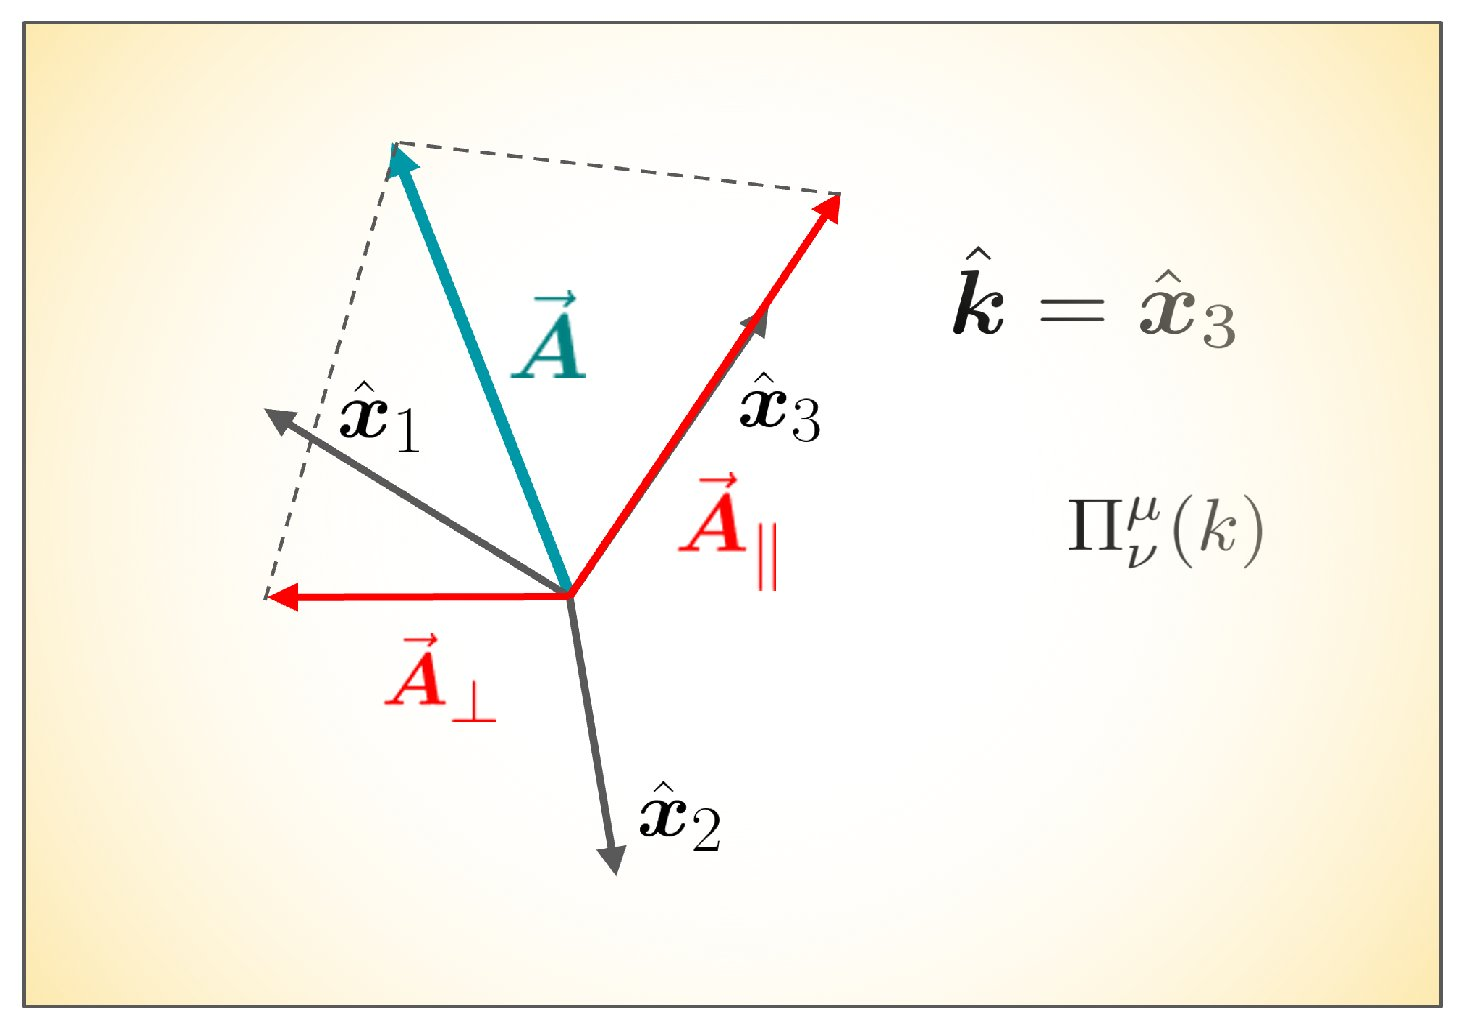
\includegraphics[width=0.55\linewidth]{plots/ChrisAxis.jpg}
    \caption{Vector potential is projected onto $\boldsymbol{\hat{k}} = \boldsymbol{\hat{x_3}} =\boldsymbol{\hat{z}}$. \radapt{Grayson:2024okq}.}
    \label{fig:project}
\end{figure}
%%%%%%%%%%%%%%%%%%%%%%%%%%

Note that the Lorentz gauge condition $\partial_\mu A^\mu = 0$ implies
\begin{equation}\label{eq:apar}
\widetilde{A}_\parallel = \frac{\omega}{ |\boldsymbol{k}|}\widetilde{\phi}\, ,
\end{equation} 
with $\phi=A^0$. The induced charge is calculated using the projected polarization tensor \req{eq:poltenmat}:
\begin{equation}
    \widetilde{\rho}_\text{ind}(\omega,\boldsymbol{k})  = \Pi^0_\nu \widetilde{A}^\nu = -\frac{|\boldsymbol{k}|^2}{\omega^2} \Pi_{\parallel}\widetilde{\phi} +  \frac{|\boldsymbol{k}|}{\omega}\Pi_{\parallel} \widetilde{A}_{\parallel}\,.
\end{equation}
For the Lorentz gauge condition \req{eq:apar}, one finds
\begin{equation}\label{eq:indch}
    \widetilde{\rho}_\text{ind}(\omega,\boldsymbol{k})  = \Pi_{\parallel}\widetilde{\phi} \left(1 -\frac{|\boldsymbol{k}|^2}{\omega^2}\right)\,.
\end{equation}
The longitudinal current is,
\begin{equation}\label{eq:indjpar}
\widetilde{j}_{\parallel\text{ind}}(\omega,\boldsymbol{k})  =  \Pi^z_\nu \widetilde{A}^\nu  = \Pi_{\parallel}  \frac{\omega}{|\boldsymbol{k}|}\widetilde{\phi}\left(1-\frac{|\boldsymbol{k}|^2}{\omega^2} \right)\,,
\end{equation}
as expected from current conservation $\partial^\mu j_\mu(x) =0$.
The induced transverse current is
\begin{equation}\label{eq:indjperp}
   \boldsymbol{j}_{\perp\text{ind}}(\omega,\boldsymbol{k})  =  \Pi_{\perp} \widetilde{A}_\perp\,.
\end{equation}
Solving for the potential on both sides of \req{eq:Amu} with the help of \reqs{eq:indch}{eq:indjperp} gives the self-consistent solutions \cite{Grayson:2022asf}
\begin{align}\label{eq:phi}
&\widetilde{\phi}(\omega,\boldsymbol{k}) = \frac{\widetilde{\rho}_\text{ext}(\omega,\boldsymbol{k})}{\varepsilon_0(\boldsymbol{k}^2-\omega^2) \left(\Pi_{\parallel}/( \omega^2\varepsilon_0)+1\right) }\,, \\\label{eq:aperp}
&\widetilde{\boldsymbol{A}}_\perp(\omega,\boldsymbol{k}) = \frac{\mu_0 \widetilde{\boldsymbol{j}}_{\perp \text{ext}}(\omega,\boldsymbol{k})}{\boldsymbol{k}^2 - \omega^2 - \mu_0 \Pi_{\perp}}\,.
\end{align}
The gauge condition \req{eq:apar} gives the self-consistent potential $\widetilde{A}_\parallel$. These self-consistent potentials determine the electric and magnetic fields via the usual relations
\begin{equation}\label{eq:ftfields}
\widetilde{\boldsymbol{B}}(\omega,\boldsymbol{k}) = i\boldsymbol{k} \times \widetilde{\boldsymbol{A}}_\perp\,, \quad \widetilde{\boldsymbol{E}}(\omega,\boldsymbol{k}) = -i \boldsymbol{k} \widetilde{\phi} + i \omega \widetilde{\boldsymbol{A}}\,.
\end{equation}
To obtain the electromagnetic fields in position space, one must Fourier transform \reqs{eq:phi}{eq:aperp}. If done analytically, this usually requires finding the poles in the denominator of these expressions, which equates to finding the poles of the thermal photon propagator. These poles represent propagating modes in the plasma. Modes will often be located at complex values in the $\omega, \mathbf{k}$ plane, leading to finite lifetimes and spatial dispersion. 

%%%%%%%%%%%%%%%%%%%%%%%%%%%%%%%%%
\para{Small back-reaction limit}
Here, we briefly mention an alternative to the self-consistent fields, which comes from assuming that the back reaction of the plasma due to the external fields is small compared to the external field. In this case, one can use the external field in the linear response equation instead of the total field
\begin{equation}\label{eq:pert}
    \widetilde{j}_{\mathrm{ind}}^{\mu}(k) = {\Pi^{\mu}}_{\nu}(k) \widetilde{A}_\text{ext}^{\nu}(k)\,.
\end{equation}
Inserting this into \req{eq:Amu} successively to find a series expansion yields the same expression as expanding \reqs{eq:phi}{eq:aperp} in the polarization functions
\begin{align}\label{eq:phipert}
&\widetilde{\phi}(\omega,\boldsymbol{k}) = \sum_{n=0}^\infty\frac{\widetilde{\rho}_\text{ext}(\omega,\boldsymbol{k})}{\varepsilon_0(\boldsymbol{k}^2-\omega^2)}\left(-\frac{\Pi_{\parallel}}{ \omega^2\varepsilon_0}\right)^n\,, \\\label{eq:aperppert}
&\widetilde{\boldsymbol{A}}_\perp(\omega,\boldsymbol{k}) = \sum_{n=0}^\infty\frac{\mu_0 \widetilde{\boldsymbol{j}}_{\perp \text{ext}}(\omega,\boldsymbol{k})}{(\boldsymbol{k}^2 - \omega^2)^{n+1}}(\mu_0 \Pi_{\perp})^{n}\,.
\end{align}
The first term $n=0$ is the vacuum field, and higher-order terms describe the back reaction of the induced current on the external field. Notably, the series expansion of \req{eq:aperp} does not accurately represent the late-time magnetic field in QGP during heavy-ion collisions\index{heavy-ion!collisions}. This is because the infinite series of \reqs{eq:phi}{eq:aperp} must be performed to capture the pole structure of the field. 

Electromagnetic fields in a polarizable medium are often described using the electric displacement field $\mathbf{D}$, the magnetic fields $\mathbf{H}$, the polarization $\mathbf{P}$, and the magnetization $\mathbf{M}$. This formulation is only useful when the field or the medium's response is static or time-dependent. When introducing spatial and temporal dispersion, these definitions are no longer unique \cite{melrose2008quantum}. For instance, if the magnetization depends on space and time $\mathbf{M}(t,x)$ the time dependence of the magnetic field generated will lead to electric fields through Faraday's Law leading to ambiguity since the displacement field no longer depends on just polarization field $\mathbf{P}$.

%%%%%%%%%%%%%%%%%%%%%%%%%%%%%%%%%
\subsection{General properties of EM fields in a plasma}
In the case of an infinite homogeneous plasma, its properties are completely described by two independent polarization functions $\Pi_\parallel(k)$ and $\Pi_\perp(k)$. In the framework presented here, the properties of these scalar functions are imparted on the electromagnetic fields via the poles in the Fourier transform of the propagators in \reqs{eq:phi}{eq:aperp}. After contour integration, one effectively gets a sum of different electromagnetic fields at each pole, the amplitude of which depends on the residue of the pole and a spacetime dependence, leading to growth attenuation or propagation depending on the pole's location. An example of this process in done in \cite{Grayson:2022asf}, where we Fourier transform the magnetic field in the center of heavy-ion collisions. 

%%%%%%%%%%%%%%%%%%%%%%%%%%%%
\para{Dispersion relation}
We can find the poles of the propagator or, equivalently, the zeros of the dispersion relation by inverting Maxwell's equations
\begin{equation}
    -ik_{\mu}\widetilde{F}^{\mu \nu} = \mu_0( \widetilde{j}_{\mathrm{ind}}^{\nu}+\widetilde{j}_{\mathrm{ext}}^{\nu})\,.
\end{equation}
Including the induced current on the left-hand side of the equation and writing the expression in terms of $A^{\mu}$ one finds
\begin{equation}
    (k^2g^{\mu \nu} - k^{\mu} k^{\nu} + \mu_0\Pi^{\mu \nu})\widetilde{A}_{\nu} = - \mu_0\widetilde{j}_{\mathrm{ext}}^{\nu} \,.
\end{equation}
The propagator $D^\mu_\nu(k)$ is obtained by inverting the previous equation
\begin{equation}
    \widetilde{A}_{\nu}(k) = -D^{\mu}_{\nu}(k) \,\widetilde{j}_{\mathrm{ext}}^{\nu}(k) \,.
\end{equation}
The poles of $D^\mu_\nu(k)$ are given by the dispersion equation~\cite{melrose2008quantum}:
\begin{equation}\label{eq:disp}
 \frac{1}{(k\cdot u)^2}\left[(k\cdot u)^2+ \mu_0\Pi_\parallel(k)\right]\left[k^2 + \mu_0 \Pi_\perp(k)\right]^2=0 \,.
\end{equation}
The transverse mode has duplicate solutions as it describes modes in a plane perpendicular to $\boldsymbol{k}$.

The dispersion \req{eq:disp} can be solved for numerous choices of variables describing the modes, such as frequency, phase velocity, or wavevector. We chose to solve for the modes of the plasma in terms of frequency $\omega_m (\mathbf{k})$, which can be thought of as a quasi-particle $m$ with energy $\omega$ and momentum $\mathbf{k}$ analogous to the usual momentum energy relation 
\begin{equation}
    E^2 = \boldsymbol{p}^2 +m^2\, ,
\end{equation}
with $c=1$. This is not always the best choice for simplifying the solutions of \req{eq:disp}, but these modes are often the easiest to interpret. A study of the modes for the general polarization tensor is not the most informative process unless one is looking for general behavior, which can be found in most plasma physics textbooks. Usually, in looking at these modes $\omega_m(\mathbf{k})$, one must first assume the external field's shape or some flow distribution in the plasma by specifying the equilibrium momentum distribution to yield interesting effects in the modes such as plasma instabilities.

When the plasma is perturbed in time in a way that doesn't depend on space, such as for a plane wave, one can take $k \to 0$ for both the transverse and longitudinal roots of the dispersion relation, which reduces the frequency of plasma oscillations \cite{Formanek:2021blc,Grayson:2022asf}
\begin{equation}\label{plasmafreq}
    \omega_{\pm} = -\frac{i\kappa}{2} \pm \sqrt{\omega_p^2 - \frac{\kappa}{4}^2}\,,
\end{equation}
the plasma frequency $\omega_p$ is explicitly given in the ultrarelativistic and nonrelativistic limits, respectively, by \cite{Formanek:2021blc}:
\begin{equation}
\omega_p^2 = \frac{1}{3} m_D^2 \quad (\mathrm{UR})\,, \qquad \omega_p^2 = m_L^2 \quad (\mathrm{NR}) \,,
\end{equation}
with
\begin{equation}
    m_D^2 = \frac{e^2 T}{3}\,.
\end{equation}
The Debye screening mass $m_D$ describes the strength of polarization in the plasma. The plasma frequency $\omega_p$ is the characteristic response frequency of the plasma. For an external field, which is an oscillatory wave of the form $E=E_0e^{-i\omega t}$, one would find that the response is weakly-damped or over-damped depending on the size of $\kappa$ according to \req{eq:plasmafreq}. Waves are weakly damped for $\kappa \ll \omega_p$, and since the square root is imaginary for $\kappa > 2\omega_p$, waves become over-damped. These general statements are subject to the spacetime dependence of the external perturbation. For instance, if a particle moves through the plasma at a constant velocity, the field will not experience much damping if the velocity is much less than the speed of sound in the plasma.

In the static limit $\omega \rightarrow 0$ the zeros in the longitudinal dispersion relation take on the form
\begin{equation}
    |\mathbf{k}| = \pm  i m_D \,.
\end{equation}
Fourier transforming using the positive root in \req{eq:phi} gives the Debye-H\"uckel screening of a stationary charge within the plasma \cite{Debye:1923}
\begin{equation}
    \phi(r) = \frac{Z \alpha \hbar c \, e^{-r/\lambda_D}}{r}\,, \quad \text{with} \quad  \lambda_D = \frac{m_D}{\hbar c}\,.
\end{equation}
The Debye length $\lambda_D$ describes the size of the polarization cloud around a charge generated by the plasma.

%%%%%%%%%%%%%%%%%%%%%%%%%%
\para{Permittivity, susceptibility, and conductivity}
In most fields of applied physics, the effects of a polarizable medium on electromagnetic fields are not described by the polarization functions $\Pi_\parallel$ and $\Pi_\perp$. It is instructive to connect these quantities to more commonplace definitions such as relative permittivity $\epsilon$, susceptibility $\chi$, and conductivity $\sigma$.

The dielectric and susceptibility tensors are related to the spatial portion of the polarization tensor $\Pi^i_j$ ~\cite{Starke:2014tfa,melrose2008quantum},
\begin{equation}\label{dielten}
     \boldsymbol{K}^i_j(\omega,\boldsymbol{k}) = \boldsymbol{\varepsilon}^i_j/\varepsilon_0 = 1+\frac{\boldsymbol{\Pi}^i_j(\omega,\boldsymbol{k})}{\omega^2} = 1+\boldsymbol{\chi}^i_j(\omega,\boldsymbol{k})\,.
\end{equation}
When we project on the axis $\mu =3$, the spatial portion of the polarization tensor is
 \begin{equation}
    \boldsymbol{\Pi}^{i}_{j}(\omega,\boldsymbol{k}) = \left[
    \begin{array}{ccc}
  \Pi_{\perp} & 0 & 0 \\
  0 & \Pi_{\perp} & 0 \\
  0& 0 & \Pi_{\parallel} \\ 
\end{array}
\right]\,.
\end{equation}
It is then natural to discuss transverse and longitudinal susceptibilities,
\begin{equation}\label{eq:chi}
    \chi_\parallel(\omega,\boldsymbol{k}) =\frac{\Pi_\parallel(\omega,\boldsymbol{k})}{\omega^2}, \quad \text{and} \quad \chi_\perp(\omega,\boldsymbol{k}) = \frac{\Pi_\perp(\omega,\boldsymbol{k})}{\omega^2}\,,
\end{equation}
and their associated permeabilities $K_\parallel$ and $K_\perp$. These quantities are useful for studying the attenuation of electromagnetic fields by looking at light absorption.

The conductivity tensor is found by taking the spatial part of the linear response equation \req{eq:ohm} and expressing the vector potential in terms of the electric field $i \omega \widetilde{A^i} = \widetilde{E^i}$~\cite{Starke:2014tfa,melrose2008quantum}
\begin{align}\label{eq:sigmaperp}
    \sigma_\perp(\omega,\boldsymbol{k}) &\equiv - i \omega \chi_\perp(\omega,\boldsymbol{k}) =- i \frac{\Pi_\perp(\omega,\boldsymbol{k})}{\omega} \,,\\
    \sigma_\parallel(\omega,\boldsymbol{k}) &\equiv - i \omega \chi_\parallel(\omega,\boldsymbol{k}) =- i \frac{\Pi_\parallel(\omega,\boldsymbol{k})}{\omega} \,.
\end{align} 
In the long wavelength limit $k \to 0$ the conductivity \req{eq:sigmaperp} reduces to \req{eq:drude}, the Drude model of conductivity~\cite{Drude:1900}.
The Drude model is equivalent to solving the Vlasov-Boltzmann equation\index{Vlasov-Boltzmann equation}  using the Anderson-Witting collision term \req{eq:lincoll} and neglecting spatial dispersion.

These quantities and results are detailed and plotted in \cite{Formanek:2021blc}. While these quantities are useful for communicating the physics of plasma response, the limits of these quantities must be taken carefully to retain the causal properties of the field. Specifically, tacitly expanding these quantities in either $\omega$ and $\mathbf{k}$ and then inserting them into the self-consistent potentials \reqs{eq:phi}{eq:aperp} will not necessarily generate causal solutions. Instead of carefully expanding and taking limits of these quantities to ensure analyticity, it's often easier to expand the electromagnetic fields within their Fourier transforms as in Appendix B of \cite{Grayson:2022asf}.


